\section{ラウンド 2--3：IRT による高速化探索}\label{sec:r2}
第 1 ラウンドでは全候補を 110 問の fitness で評価しており（1 候補あたり生成だけで約 1,000 秒），EvoGM の外側ループに回す予算が残らなかった．そこで追加の上限 GPU 8 時間のもとで探索を続けるため，保存した探索状態から再開し，全問評価の大半を安価な推定値に置き換えた．

\paragraph{IRT サブセットと推定量．}ラウンド 1 の 40 候補 $\times$ 110 問の正誤行列（打ち切り＝不正解）に，タスク（MMLU-Pro，GPQA，BFCL）ごとの 2PL 項目反応モデルを同時 MAP 推定で当てはめた（$\theta\sim\mathcal N(0,1)$，$\log a\sim\mathcal N(0,0.5^2)$，$b\sim\mathcal N(0,2^2)$）．タスクごとに，上位 15 候補の能力値における Fisher 情報量を $\sqrt{\text{平均トークン数}}$ で割った値が大きい問題を残した．MMLU-Pro 16 問，GPQA 10 問，BFCL 14 問の計 40 問である（1 候補あたり約 6.6 万トークン．全問では約 16.5 万）．新しい候補はこの 40 問だけに回答する．タスクごとの fitness 推定値は，サブセットでの正答数に，未観測の問題に対する 2PL 確率 $p(\theta_{\text{MAP}})$ の和を足し，タスクの問題数で割ったものである．3 タスクの値を平均するので，推定値はラウンド 1 の fitness と同じ尺度になる．ラウンド 1 の 40 候補での一個抜き検証では，全問 fitness に対する平均絶対誤差（MAE）が 0.013（上位 15 候補では 0.009），順位相関が 0.93 だった．サブセットの単純な正答率では MAE 0.066 である．

\paragraph{レーシング．}生成中の出力を逐次受け取り，サブセットの半分以上が終わった時点で楽観的な推定値（$\theta+1.5\,\text{sd}$）を計算する．これが現在の集団の $P$ 番目の値を下回れば，その候補の生成を打ち切る．ラウンド 1 の反復 2--3 を使ったオフラインのシミュレーションでは，20 候補中 4 候補を打ち切り，時間を約 9\% 節約し，誤って打ち切った候補はなかった．

\paragraph{完全評価のルール．}推定誤差と勝者の呪いに備え，各反復の後に，まだ完全評価していない集団メンバーのうち最良のものの推定値が，それまでの最良の厳密 fitness から 0.02 以内であれば，上位 2 メンバーを残り 70 問で評価した（GPU 1 枚に 1 候補）．これでラウンド 1 と同じ定義の厳密な 110 問 fitness が得られる．集団と生成器には，得られている最良の値（厳密値があればそれ，なければ推定値）を使う．最終的な勝者は，ラウンド 1 と全ての完全評価を通じて\textbf{厳密な} 110 問 fitness が最大の候補であり，180 問テストはその候補だけで行う．

\paragraph{探索の進め方．}各ラウンドの最初に基底を入れ替える．前ラウンドまでの履歴の上位 8 候補が新しいエキスパートとなり（ラウンド 2 では fitness .722，.703，.697，.697，.692，.692，.689，.686），探索はその座標系で行う．$P=10$，生成器はラウンドごとに初期化し，ラウンドあたり最大 3 反復とした．ラウンドと反復の数は，計測したコストからカーネル内で決め，最終テストの時間は常に確保した．

\section{ラウンド 2--3：結果}\label{sec:r2res}
\paragraph{実行．}実行は 2$\times$T4 で GPU 6.53 時間（上限 8 時間）で終わった．ラウンド 2 と 3 をそれぞれ 3 反復で完了し，ラウンド 4 は残り 0.88 時間が 1 ラウンドの最低所要 0.92 時間に満たないため省略した．新規のサブセット評価は 64 回（ラウンド 1 と合わせて計 104 候補），完全評価は 12 回で，レーシングで途中打ち切りになった候補は 3，失敗した候補は 0 だった．

\paragraph{探索の推移．}最良の厳密 fitness はラウンド 2 の間はラウンド 1 の値 0.722 のままで（完全評価した候補の 1 つが同点），ラウンド 3 の反復 2 で 0.733，反復 3 で 0.764 に上がった（図\ref{fig:search}左）．完全評価した 12 候補では，IRT 推定値と厳密 fitness の MAE は 0.009，Spearman 相関は 0.96，平均バイアスは $+0.008$ だった（図\ref{fig:search}右）．推定値が高いものを選んで完全評価しているので，このバイアスは想定どおりである．最も顕著なのは勝者で，推定値 0.782 に対し厳密 fitness は 0.764 だった．

\begin{figure}[htbp]
\centering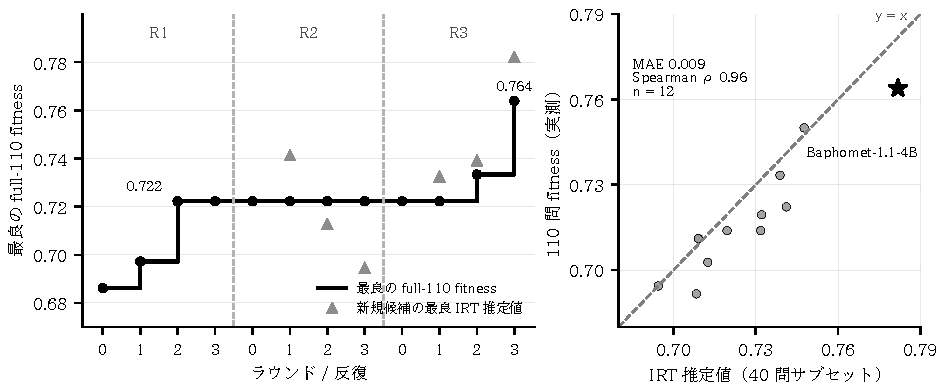
\includegraphics[width=\textwidth]{fig_search_r2_ja.pdf}
\caption{左：ラウンド 1--3 の各反復後の，その時点までの最良の厳密 110 問 fitness（反復 0＝そのラウンドの初期集団）．三角は各反復の新規候補のうち最良の IRT 推定値（ラウンド 2--3）．右：完全評価した 12 候補の IRT 推定値と厳密 110 問 fitness．星が Baphomet-1.1-4B．}
\label{fig:search}
\end{figure}

\paragraph{Baphomet-1.1-4B の係数．}ラウンド 3 の勝者の係数は
\begin{align*}\lambda_{1.1} = (&0.0116,\ 0.2039,\ 0.5901,\ 0.0013,\ 0.2972,\ 0.0323,\ 0.0030,\ -0.0007)\end{align*}
で（順に Agents-A1，dsv4pro，q38distill，Qwopus-Coder，Qwopus-v3，AREX-Turbo，NeoHorse，T-Max），$\sum\lambda_i=1.14$ である．ラウンド 1 勝者と同じ 3 ドナーを使いつつ，q38distill（0.63\,$\to$\,0.59）から dsv4pro（0.10\,$\to$\,0.20）と Qwopus-v3（0.23\,$\to$\,0.30）へ重みを移している．残り 5 ドナーはほぼ 0 のままである（図\ref{fig:lambda}）．

\begin{figure}[htbp]
\centering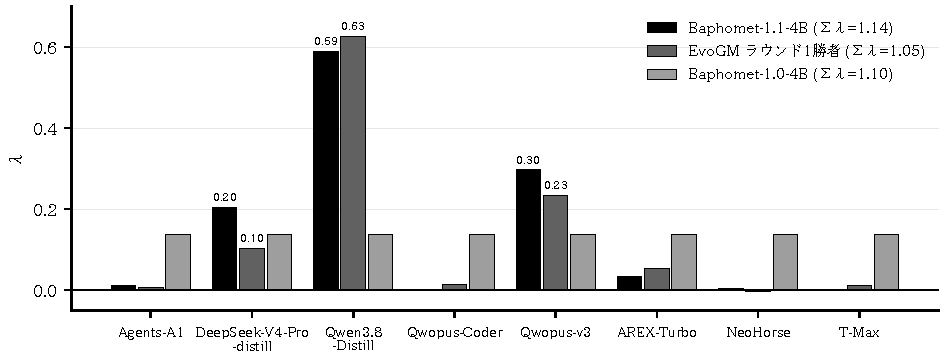
\includegraphics[width=\textwidth]{fig_lambda_ja.pdf}
\caption{Baphomet-1.1-4B，ラウンド 1 勝者，Baphomet-1.0-4B のマージ係数．}
\label{fig:lambda}
\end{figure}

\paragraph{fitness セットでのエキスパートとの比較．}表\ref{tab:fit110}と図\ref{fig:fit110}--\ref{fig:fit110eff}に，110 問の fitness 用問題（上限 4,096 トークン）での Baphomet-1.1，8 つのドナー，均等平均，Baphomet-1.0，ラウンド 1 勝者の比較を示す．Baphomet-1.1 の fitness が最も高く（0.764），最良の単体ドナー（q38distill，0.686）を 0.078，Baphomet-1.0（0.603）を 0.161 上回る．MMLU-Pro（.800）と GPQA（.567）では 1 位または同率 1 位だが，BFCL では AREX-Turbo の方が高い（.950 対 .925）．注意点が二つある．Baphomet-1.1 はこの問題で\textbf{選ばれた}モデルなので，そのスコアは楽観的に偏っている（ドナーのスコアにはこの偏りはない）．また，ドナーはこのセットでのみ評価しており，180 問テストでは\textbf{評価していない}．

\begin{table}[htbp]
\centering\small
\caption{110 問 fitness セット（上限 4,096 トークン）．fitness＝3 タスクの正答率の平均，打切＝打ち切られた回答の割合（\%），トークン＝平均生成トークン数．Baphomet-1.1 とラウンド 1 勝者はこの問題で選ばれた（楽観的）．ドナーは 180 問テストでは未評価．}
\label{tab:fit110}
\setlength{\tabcolsep}{3.5pt}
\begin{tabular}{lcccrrr}
\toprule
モデル & MMLU & GPQA & BFCL & fitness & 打切 & トークン \\
\midrule
\textbf{Baphomet-1.1-4B} & .800 & .567 & .925 & \textbf{.764} & 11.8 & 1,149 \\
ラウンド 1 勝者 & .800 & .467 & .900 & .722 & 12.7 & 1,096 \\
\midrule
q38distill & .700 & .433 & .925 & .686 & 3.6 & 671 \\
dsv4pro & .675 & .467 & .850 & .664 & 19.1 & 1,331 \\
Qwopus-v3 & .700 & .233 & .925 & .619 & 27.3 & 1,835 \\
Qwopus-Coder & .650 & .167 & .875 & .564 & 33.6 & 1,834 \\
NeoHorse & .600 & .033 & .900 & .511 & 40.0 & 2,180 \\
T-Max & .500 & .133 & .900 & .511 & 41.8 & 2,343 \\
AREX-Turbo & .425 & .067 & .950 & .481 & 28.2 & 1,924 \\
Agents-A1 & .450 & .067 & .750 & .422 & 48.2 & 2,492 \\
\midrule
Baphomet-1.0-4B & .650 & .233 & .925 & .603 & 31.8 & 1,925 \\
均等平均（$1/8$） & .675 & .200 & .900 & .592 & 30.9 & 2,073 \\
\bottomrule
\end{tabular}
\end{table}

\begin{figure}[htbp]
\centering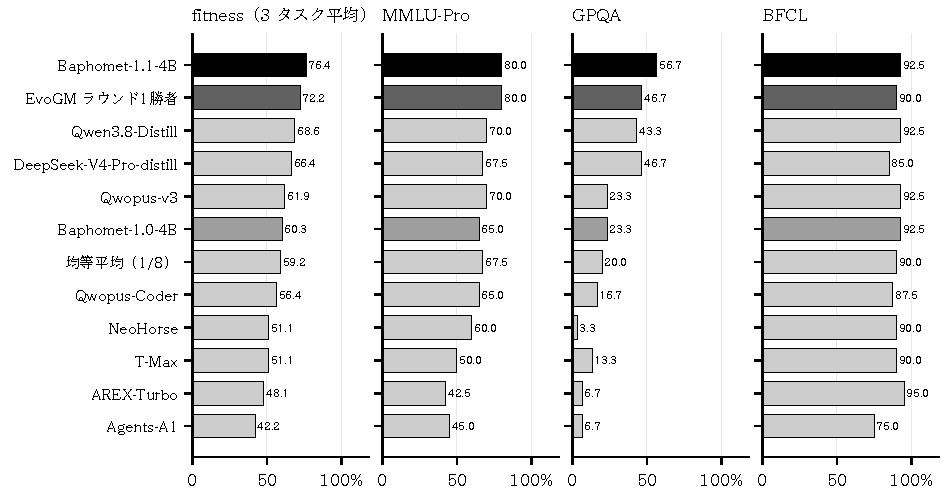
\includegraphics[width=\textwidth]{fig_fit110_acc_ja.pdf}
\caption{110 問 fitness セットにおける fitness とタスク別正答率（Baphomet-1.1-4B，ラウンド 1 勝者，8 ドナー，Baphomet-1.0-4B，均等平均）．Baphomet-1.1 はこの問題で選ばれたため，そのスコアは楽観的である．}
\label{fig:fit110}
\end{figure}

\begin{figure}[htbp]
\centering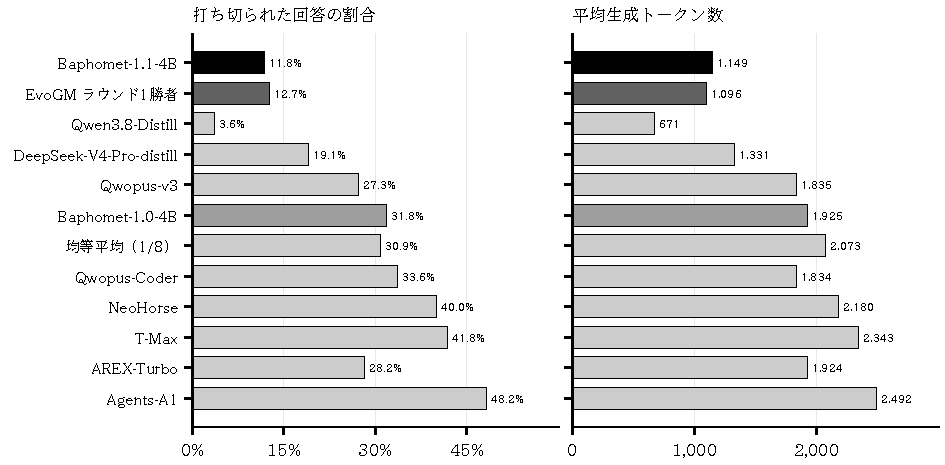
\includegraphics[width=\textwidth]{fig_fit110_eff_ja.pdf}
\caption{110 問 fitness セットにおける打ち切り率と平均生成トークン数（モデルと順序は図\ref{fig:fit110}と同じ）．}
\label{fig:fit110eff}
\end{figure}

\paragraph{テスト．}テストで評価した 4 モデルの 180 問の結果を表\ref{tab:test}と図\ref{fig:test}に示す（ドナーと均等平均は未評価）．Baphomet-1.1 は全体で数値上最も高く（79.4\%，Wilson 95\% 信頼区間 73.0--84.7），Baphomet-1.0（77.8\%，71.2--83.2），ラウンド 1 勝者（77.2\%，70.6--82.7），Qwen3.5-4B（70.0\%，62.9--76.2）が続く．信頼区間は大きく重なっている．対応のある検定（表\ref{tab:mcnemar}）では，Baphomet-1.1 は Baphomet-1.0（勝ち 10 問，負け 7 問，$p=0.63$）にもラウンド 1 勝者（12 対 8，$p=0.50$）にも\textbf{有意には}勝っていない．基盤モデルには有意に勝っており（20 対 3，$p<0.001$），主に GPQA（10 対 0，$p=0.002$）と MMLU-Pro（9 対 1，$p=0.021$）による．Baphomet-1.0 に対するスイート別の差は MMLU-Pro で +3.8 ポイント，GPQA で +4.0，BFCL で $-4.0$（不一致ペア 0 対 2）で，いずれも有意ではない．

\begin{table}[htbp]
\centering\small
\caption{180 問テスト（上限 8,192 トークン）．正答率は\%，打切＝打ち切られた回答の割合（\%），トークン＝平均生成トークン数．ドナーはこのテストでは未評価．}
\label{tab:test}
\setlength{\tabcolsep}{4pt}
\begin{tabular}{llrrr}
\toprule
スイート（$n$） & モデル & 正答率 & 打切 & トークン \\
\midrule
MMLU-Pro（80） & \textbf{Baphomet-1.1-4B} & \textbf{81.3} & 5.0 & 1,492 \\
 & ラウンド 1 勝者 & 75.0 & 5.0 & 1,200 \\
 & Baphomet-1.0-4B & 77.5 & 13.8 & 3,331 \\
 & Qwen3.5-4B & 71.3 & 17.5 & 4,385 \\
\midrule
GPQA（50） & \textbf{Baphomet-1.1-4B} & \textbf{62.0} & 28.0 & 4,007 \\
 & ラウンド 1 勝者 & 62.0 & 16.0 & 3,270 \\
 & Baphomet-1.0-4B & 58.0 & 34.0 & 5,915 \\
 & Qwen3.5-4B & 42.0 & 54.0 & 7,094 \\
\midrule
BFCL（50） & \textbf{Baphomet-1.1-4B} & 94.0 & 0.0 & 207 \\
 & ラウンド 1 勝者 & 96.0 & 0.0 & 202 \\
 & Baphomet-1.0-4B & \textbf{98.0} & 0.0 & 205 \\
 & Qwen3.5-4B & 96.0 & 0.0 & 229 \\
\midrule
全体（180） & \textbf{Baphomet-1.1-4B} & \textbf{79.4} & 10.0 & 1,834 \\
 & ラウンド 1 勝者 & 77.2 & 6.7 & 1,498 \\
 & Baphomet-1.0-4B & 77.8 & 15.6 & 3,180 \\
 & Qwen3.5-4B & 70.0 & 22.8 & 3,983 \\
\bottomrule
\end{tabular}
\end{table}

\begin{table}[htbp]
\centering\small
\caption{180 問テストでの対応のある比較．前者だけが正解した問題数--後者だけが正解した問題数と，正確な両側 McNemar 検定の $p$ 値．}
\label{tab:mcnemar}
\setlength{\tabcolsep}{4pt}
\begin{tabular}{lcccc}
\toprule
比較 & 全体 & MMLU-Pro & GPQA & BFCL \\
\midrule
Baphomet-1.1 対 Baphomet-1.0 & 10--7（$p$=.63） & 5--2（.45） & 5--3（.73） & 0--2（.50） \\
Baphomet-1.1 対 ラウンド 1 勝者 & 12--8（.50） & 7--2（.18） & 5--5（1.0） & 0--1（1.0） \\
Baphomet-1.1 対 Qwen3.5-4B & 20--3（$<$.001） & 9--1（.021） & 10--0（.002） & 1--2（1.0） \\
ラウンド 1 勝者 対 Baphomet-1.0 & 8--9（1.0） & 3--5（.73） & 5--3（.73） & 0--1（1.0） \\
Baphomet-1.0 対 Qwen3.5-4B & 17--3（.003） & 7--2（.18） & 9--1（.021） & 1--0（1.0） \\
\bottomrule
\end{tabular}
\end{table}

\begin{figure}[htbp]
\centering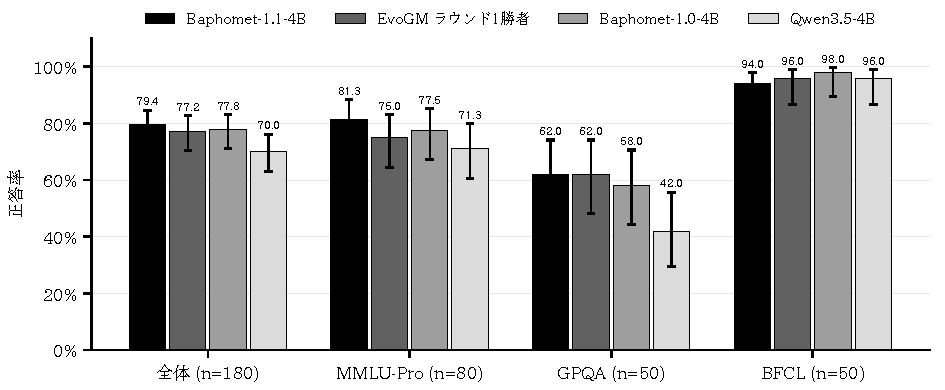
\includegraphics[width=\textwidth]{fig_test180_acc_ja.pdf}
\caption{180 問テストの正答率と Wilson 95\% 信頼区間（上限 8,192 トークン）．テストで評価したのはこの 4 モデルのみで，8 ドナーと均等平均は未評価．}
\label{fig:test}
\end{figure}

\paragraph{推論の長さ．}Baphomet-1.1 の生成トークン数は Baphomet-1.0 より全体で 42\% 少なく（1,834 対 3,180．MMLU-Pro で 55\%，GPQA で 32\% 少ない），打ち切りも少ない（10.0\% 対 15.6\%）．一方，ラウンド 1 勝者と比べると長く（1,834 対 1,498 トークン），打ち切りも多い（10.0\% 対 6.7\%）．その差はほぼ GPQA によるものである（打ち切り 28\% 対 16\%．図\ref{fig:testeff}）．ラウンド 1 勝者に対する正答率の上積みの一部は，推論が長くなったことと引き換えに得られている．

\begin{figure}[htbp]
\centering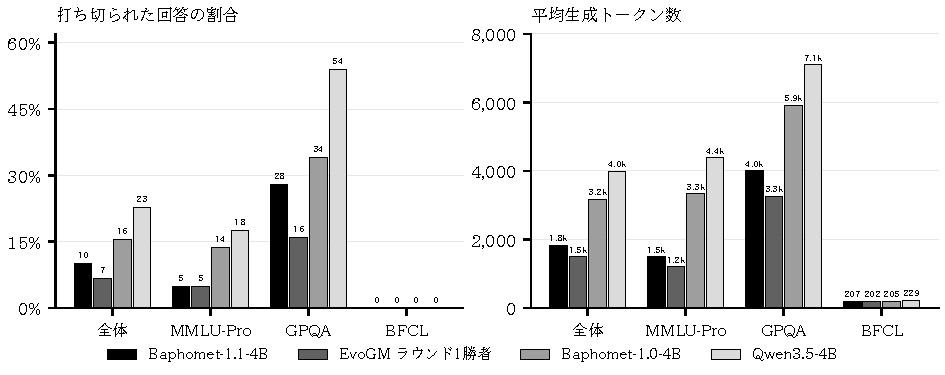
\includegraphics[width=\textwidth]{fig_test180_eff_ja.pdf}
\caption{180 問テストにおける打ち切り率と平均生成トークン数．}
\label{fig:testeff}
\end{figure}

